\documentclass[12pt, journal]{IEEEtran}
\usepackage{cite}
\usepackage{amsmath}
\usepackage{algorithmic}
\usepackage{array}
\usepackage{hyperref}
\usepackage{orcidlink}
\usepackage{stfloats}
\usepackage{graphicx}
\usepackage{float}

\bibliographystyle{IEEEtran}

\usepackage[caption=false,font=footnotesize]{subfig}

\begin{document}

\markboth{Análisis de Señales Mixtas, IS 2026}{}

\title{Análisis de Señales Mixtas \\ \textit{Diseño de un sistema de compresión espectral adaptativa en tiempo real}}

\author{
\IEEEauthorblockA{\\Escuela de Ingeniería en Computadores}
\IEEEauthorblockA{\\Instituto Tecnológico de Costa Rica} \\
\vspace{\baselineskip}\\
\IEEEauthorblockN{
Camila Lizano Brenes, 2024255324 \\
Dylan Guerrero Gonzalez, 2022016016 \\
Javier Hernandez Castillo, 2022321746 \\
Sergio Daniel Alvarez Chanto, 2024134332}
}

\maketitle

\begin{abstract}
This paper presents the design and partial implementation of a real-time adaptive spectral compression system based on the Fast Fourier Transform (FFT). The work covers the experimental stages of the project: implementation and analysis of the Discrete Fourier Transform (DFT) and FFT algorithms in a computational environment, as well as adaptive spectral compression and reconstruction using the Inverse FFT (IFFT). The compression strategy leverages Parseval's theorem to identify the minimum number of spectral components required to preserve at least 95\% of total signal energy. Experimental results demonstrate that while high energy preservation is achieved with a significantly reduced number of coefficients, this criterion does not necessarily guarantee perceptual fidelity, especially for broadband signals such as speech, where low-energy components carry relevant intelligibility information.
\end{abstract}

\begin{IEEEkeywords}
Compresor, energía, transformada de Fourier, series de Fourier.
\end{IEEEkeywords}

\section{Introduction}

El objetivo de este proyecto es diseñar e implementar un sistema de compresión y reconstrucción espectral adaptativo en tiempo real, utilizando la Transformada Rápida de Fourier (FFT) y la Transformada Inversa Rápida de Fourier (IFFT). El sistema completo opera sobre tres microcontroladores con funciones diferenciadas. El primero actúa como transmisor: captura una señal analógica mediante un ADC, calcula su FFT y aplica compresión espectral adaptativa conservando únicamente las componentes de mayor energía, para luego transmitir los coeficientes seleccionados. El segundo microcontrolador (Receptor 1) reconstruye la señal en el dominio del tiempo aplicando la IFFT y la reproduce mediante DAC o PWM filtrado, permitiendo verificar auditivamente la similitud con la original. El tercer microcontrolador (Receptor 2) también reconstruye la señal, pero con el propósito de calcular métricas cuantitativas de calidad: Error Cuadrático Medio (MSE), energía preservada y relación señal a error (SNR), mostrando los resultados en una pantalla LCD.

Debido a la naturaleza matemática del problema, el desarrollo inicia con una etapa experimental en computador, donde se implementan y analizan los algoritmos antes de llevarlos al hardware. Este proceso se refleja en la estructura del presente documento: primero se expone el marco teórico con los conceptos fundamentales, luego los resultados y análisis de los experimentos realizados, seguido de las conclusiones y finalmente las mejoras propuestas.

\section{Marco teórico}

Las series de Fourier permiten expresar cualquier señal periódica como una suma de exponenciales complejas, lo que facilita su análisis en el dominio de la frecuencia \cite{tello2016introduccion}. Esta representación resulta de gran utilidad en el procesamiento digital de señales, especialmente en aplicaciones de compresión espectral donde es necesario identificar y conservar las componentes de mayor energía.

Esto es posible gracias a la propiedad de ortogonalidad, que establece que las funciones base de distintas frecuencias son linealmente independientes entre sí. Como consecuencia, el producto interno entre funciones de distinta frecuencia es nulo, lo que permite separar y analizar cada componente espectral de forma independiente, sin interferencia entre ellas \cite{Oppenheim_Willsky_Nawab_1997}.

Para señales discretas de longitud finita, la Transformada Discreta de Fourier (DFT) obtiene la representación frecuencial a partir de muestras igualmente espaciadas. Matemáticamente, la DFT transforma la secuencia temporal $x(n)$ en un conjunto de coeficientes complejos $X(k)$ definidos como:
\begin{equation}
X(k) = \sum_{n=0}^{N-1} x(n)e^{-j2\pi kn/N}, \quad k = 0,1,\dots,N-1
\end{equation}
y la transformada inversa (IDFT) permite reconstruir la señal original a partir de dichos coeficientes:
\begin{equation}
x(n) = \frac{1}{N} \sum_{k=0}^{N-1} X(k)e^{j2\pi kn/N}
\end{equation}
Esta representación caracteriza completamente la señal en el dominio frecuencial, permitiendo identificar cómo se distribuye su energía en cada componente \cite{proakis2007digital}.

Desde el punto de vista energético, la DFT cumple con el teorema de Parseval, que establece la equivalencia entre la energía en el dominio del tiempo y en el dominio de la frecuencia:
\begin{equation}
\sum_{n=0}^{N-1} |x(n)|^2 = \frac{1}{N} \sum_{k=0}^{N-1} |X(k)|^2
\end{equation}
Esta propiedad es fundamental para la compresión espectral, ya que permite cuantificar la contribución energética de cada coeficiente y seleccionar el subconjunto mínimo que concentre la mayor parte de la energía total de la señal \cite{proakis2007digital}.

La Transformada Rápida de Fourier (FFT) es un conjunto de algoritmos que calculan la DFT de forma eficiente, reduciendo su complejidad computacional de $O(N^2)$ a $O(N \log N)$ \cite{rj2003fourier}. Esta reducción hace viable el análisis espectral en aplicaciones en tiempo real. En el contexto del proyecto, la FFT permite identificar y seleccionar las componentes de mayor energía de manera eficiente, habilitando la compresión y reconstrucción espectral en tiempo real sobre hardware embebido.

\section{Resultados y análisis}

En esta sección se presentan los resultados de los experimentos realizados en Python para la implementación de la DFT, la FFT y el sistema de compresión espectral adaptativa.

\subsection{Experimentos con FFT}

El objetivo de esta etapa fue comparar la DFT y la FFT desde el punto de vista computacional y verificar la equivalencia de sus representaciones espectrales. Se generaron señales discretas de prueba —tonos senoidales y señales multicomponente— y se calculó el espectro de cada una con ambos métodos, midiendo los tiempos de ejecución para distintos tamaños de señal $N$.

\subsubsection{Implementación de la DFT}

La DFT fue implementada directamente a partir de su definición matemática, utilizando sumatorias complejas para cada coeficiente espectral. Esta implementación permite analizar detalladamente el proceso de transformación desde el dominio del tiempo hacia el dominio de la frecuencia. Para validarla, se utilizó una señal multicomponente formada por la suma de varias senoidales de distintas frecuencias, obteniendo su espectro de magnitud.

\begin{figure}[H]
\centering
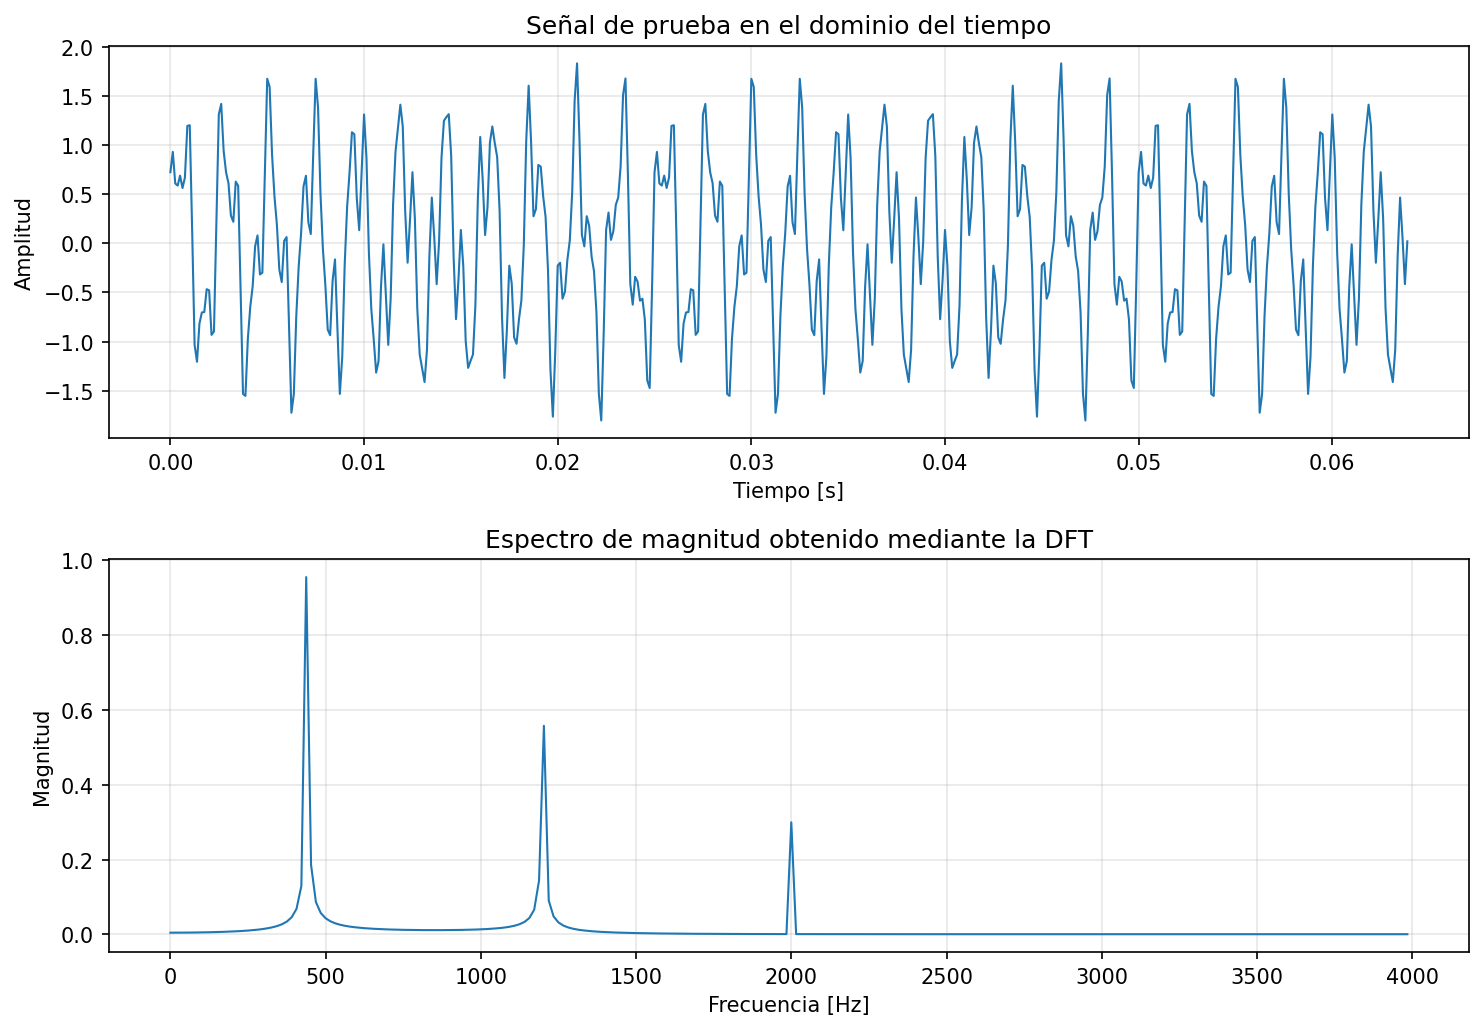
\includegraphics[width=0.48\textwidth]{dft_resultado.png}
\caption{Señal de prueba en el dominio del tiempo y espectro de magnitud obtenido mediante DFT.}
\label{fig:dft}
\end{figure}

En la Figura~\ref{fig:dft} se observan picos claramente definidos en las frecuencias correspondientes a las componentes de la señal de prueba, lo cual valida el correcto funcionamiento de la implementación de la DFT.

\subsubsection{Implementación de la FFT}

La FFT fue implementada utilizando la función optimizada de la biblioteca NumPy, basada en el algoritmo de Cooley-Tukey. Se utilizó la misma señal multicomponente que en la implementación de la DFT para garantizar una comparación directa y justa entre ambos métodos.

\begin{figure}[H]
\centering
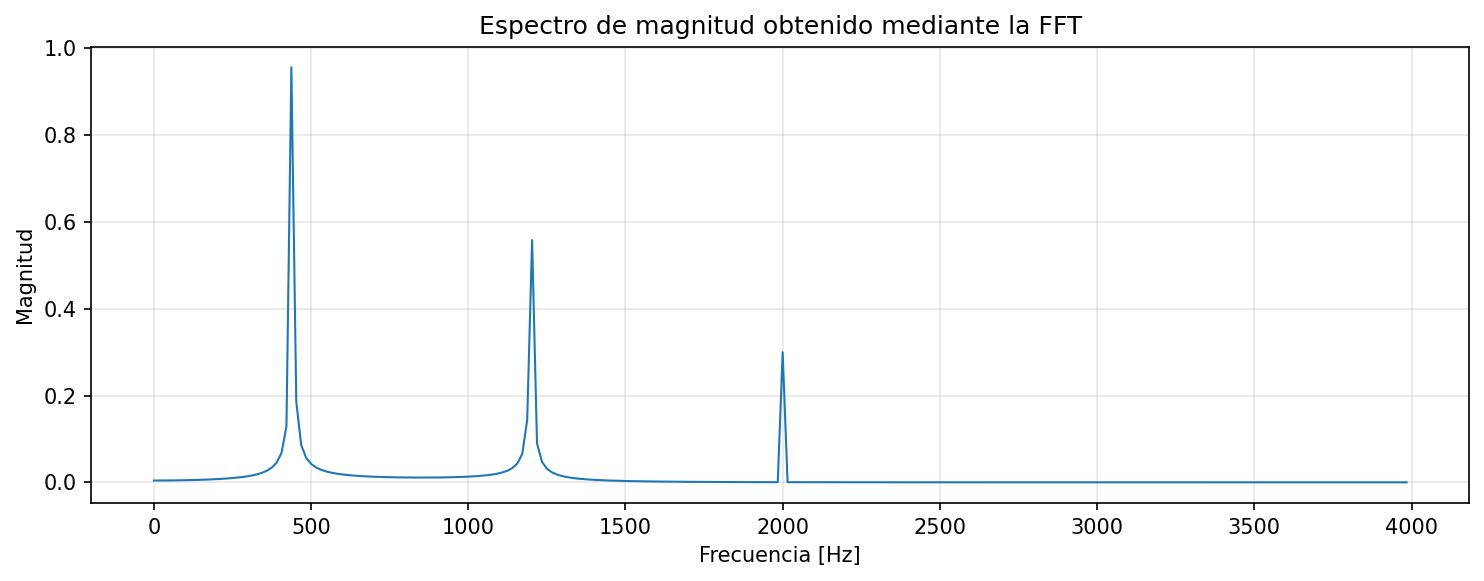
\includegraphics[width=0.48\textwidth]{fft_resultado.png}
\caption{Espectro de magnitud obtenido mediante FFT para la misma señal de prueba.}
\label{fig:fft}
\end{figure}

Como se observa en la Figura~\ref{fig:fft}, la FFT produce un espectro prácticamente idéntico al obtenido con la DFT, confirmando que ambas transformadas describen la misma información espectral. La diferencia fundamental entre ambas radica exclusivamente en su eficiencia computacional.

\subsubsection{Comparación de tiempos de ejecución}

Se realizó una comparación sistemática del tiempo de ejecución entre la DFT directa y la FFT optimizada para múltiples valores de $N$, permitiendo analizar cómo varía el rendimiento de cada método en función del tamaño de la señal.

\begin{figure}[H]
\centering

\includegraphics[width=0.48\textwidth]{tiempos_dft_fft.png}
\caption{Comparación de tiempos de ejecución entre DFT y FFT para distintos tamaños de señal.}
\label{fig:tiempos}
\end{figure}

\begin{table}[H]
\centering
\caption{Comparación de tiempos de ejecución entre DFT y FFT}
\label{tab:tiempos}
\begin{tabular}{c|c|c|c}
\hline
N & DFT [s] & FFT [s] & Relación DFT/FFT \\
\hline
64   & 0.0051 & 0.00005 & 95.41 \\
128  & 0.0223 & 0.00008 & 264.84 \\
256  & 0.0877 & 0.00007 & 1257.43 \\
512  & 0.3293 & 0.00007 & 4344.59 \\
1024 & 1.3340 & 0.00008 & 16269.10 \\
\hline
\end{tabular}
\end{table}

Como se aprecia en la Tabla~\ref{tab:tiempos} y la Figura~\ref{fig:tiempos}, el tiempo de ejecución de la DFT crece rápidamente conforme aumenta $N$, mientras que la FFT mantiene tiempos prácticamente constantes en el rango evaluado. La relación entre ambos métodos supera $10^4$ para $N = 1024$, evidenciando experimentalmente la diferencia de complejidad: $O(N^2)$ para la DFT frente a $O(N \log N)$ para la FFT. Adicionalmente, esta diferencia de rendimiento no es constante sino que aumenta con el tamaño de señal, comportamiento consistente con el análisis teórico de complejidad. Este resultado es crítico para el sistema propuesto, ya que confirma que la FFT es indispensable para garantizar el procesamiento en tiempo real.

\subsubsection{Análisis espectral: magnitud y fase}

El análisis espectral completo requiere considerar tanto la magnitud como la fase de los coeficientes de Fourier, ya que ambas juntas proporcionan la representación completa de la señal en el dominio de la frecuencia.

\begin{figure}[H]
\centering
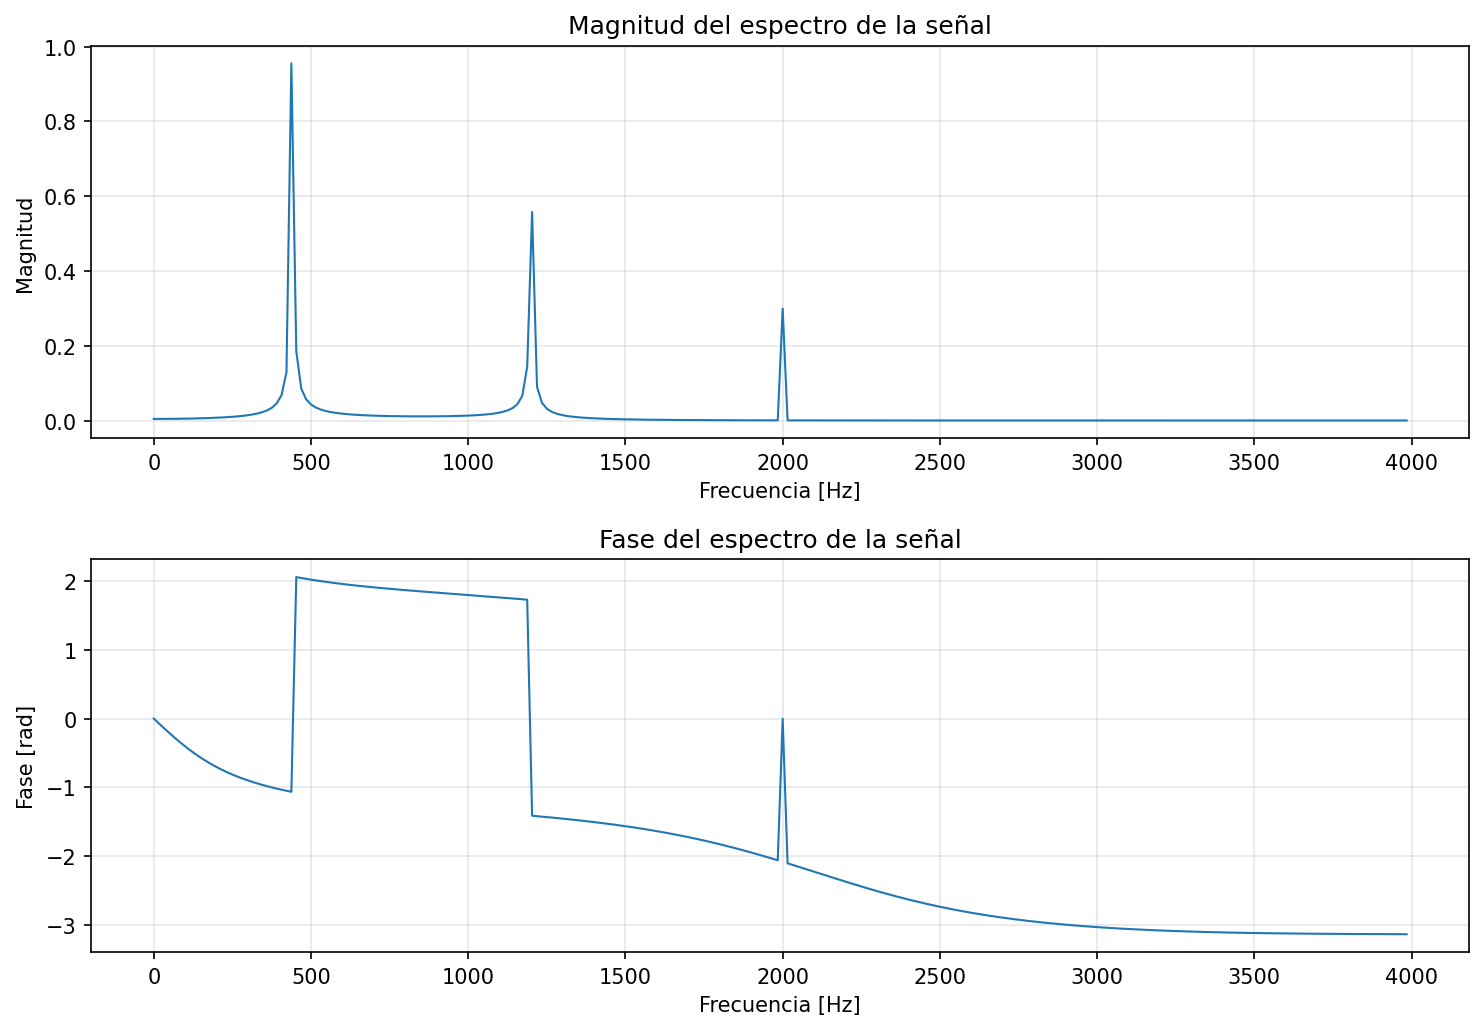
\includegraphics[width=0.48\textwidth]{magnitud_fase.png}
\caption{Magnitud y fase del espectro de la señal de prueba.}
\label{fig:fase}
\end{figure}

En la Figura~\ref{fig:fase}, la magnitud permite identificar las frecuencias dominantes presentes en la señal. La fase, por su parte, describe el desplazamiento relativo de cada componente frecuencial respecto a un origen de referencia. Conservar correctamente la información de fase es igualmente esencial para la reconstrucción precisa de la señal en el dominio del tiempo, ya que errores en la fase alteran la forma de onda reconstruida independientemente de que la magnitud sea correcta.

\subsection{Experimentos de compresión espectral}

Para la etapa de compresión, se desarrolló un sistema en Python que captura audio en tiempo real mediante micrófono a una frecuencia de muestreo de 44.1~kHz. La señal es preprocesada eliminando la componente DC y normalizando la amplitud. Con el fin de garantizar compatibilidad con el algoritmo FFT tipo Cooley-Tukey, la señal es recortada a un tamaño $N = 2^k$, correspondiente a la mayor potencia de dos menor o igual al número total de muestras capturadas.

Una vez obtenida la FFT de la señal, se calcula la energía espectral de cada coeficiente mediante el teorema de Parseval. Los coeficientes son ordenados de mayor a menor energía y se seleccionan iterativamente hasta que la energía acumulada alcanza al menos el 95\% de la energía total de la señal. Este criterio adaptativo determina de forma automática el número mínimo de componentes necesarias para representar la señal con el nivel de fidelidad predefinido.

El umbral del 95\% fue seleccionado como un equilibrio entre compresión y calidad de reconstrucción. Valores menores —como 90\%— permiten mayor reducción en el número de coeficientes pero introducen una degradación más evidente en la señal reconstruida. Por el contrario, valores más altos —como 99\%— mejoran la calidad pero reducen significativamente la eficiencia de compresión. Finalmente, se construye un espectro comprimido en el que únicamente se conservan los coeficientes seleccionados —el resto se anula— y la señal se reconstruye en el dominio del tiempo mediante la IFFT.

\subsubsection{Métricas de desempeño}

Para evaluar la calidad de la reconstrucción se calcularon las siguientes métricas: Error Cuadrático Medio (MSE), energía preservada (\%) y Relación Señal a Ruido (SNR). Los resultados obtenidos muestran que se logró preservar aproximadamente el 95\% de la energía total con un número de coeficientes significativamente menor al total disponible. El MSE fue bajo, indicando que el error promedio entre la señal original y la reconstruida es reducido desde el punto de vista energético. El valor de SNR refleja que, aunque la señal reconstruida conserva su estructura general, existe una degradación perceptual moderada, especialmente pronunciada en señales de voz, donde componentes de baja energía contienen información relevante para la inteligibilidad.

\subsubsection{Análisis gráfico}

\begin{figure}[H]
\centering

\includegraphics[width=\linewidth]{compresion_espectral.png}
\caption{Resultados de la compresión espectral: comparación entre señal original y reconstruida, espectros de magnitud, energía acumulada y error de reconstrucción.}
\label{fig:compresion}
\end{figure}

En la Figura~\ref{fig:compresion} se presenta la comparación entre la señal original y la señal reconstruida en el dominio del tiempo. Se observa que la señal reconstruida conserva la estructura general, pero presenta pérdida de detalle en regiones de mayor variabilidad o transiciones complejas. Los espectros de magnitud antes y después de la compresión muestran claramente que únicamente se conservan las componentes de mayor energía, mientras que el resto es eliminado. La curva de energía acumulada ilustra el criterio de selección utilizado para alcanzar el umbral del 95\%, y la gráfica del error de reconstrucción confirma que las diferencias entre señal original y reconstruida no están distribuidas uniformemente, sino que se concentran principalmente en los segmentos de mayor variabilidad de la señal.

En señales de tipo tonal, donde la energía se concentra en pocas frecuencias, el método resulta altamente eficiente y logra una reconstrucción prácticamente indistinguible de la original. Sin embargo, en señales de voz o banda ancha, la energía se distribuye en un mayor número de componentes espectrales, incluyendo componentes de baja energía que contienen información relevante para la inteligibilidad. La eliminación de estas componentes puede generar pérdida de detalle perceptual, afectando la calidad percibida de la señal reconstruida a pesar de haber preservado el 95\% de la energía total. Esto evidencia que la energía espectral, si bien es un criterio adecuado y eficiente para la compresión, no es suficiente por sí sola para garantizar fidelidad perceptual en aplicaciones de audio general. En aplicaciones reales, sería necesario complementar este enfoque con modelos perceptuales o técnicas de ponderación espectral.

\section{Conclusiones}

En este trabajo se implementaron y compararon la DFT y la FFT, comprobando experimentalmente que ambas producen representaciones espectrales equivalentes. Sin embargo, la diferencia de rendimiento entre ambas no es constante, sino que crece con el tamaño de la señal, lo cual es consistente con sus respectivas complejidades computacionales ($O(N^2)$ para la DFT y $O(N \log N)$ para la FFT). Este comportamiento confirma que la FFT es la herramienta adecuada para el procesamiento en tiempo real requerido por el sistema propuesto.

Se desarrolló un sistema de compresión espectral adaptativa basado en la conservación del 95\% de la energía total, logrando reducir considerablemente el número de coeficientes necesarios para representar la señal. Los resultados demuestran que el criterio energético es eficiente para señales tonales, pero presenta limitaciones en señales de voz o banda ancha, donde la preservación de energía no garantiza una reconstrucción perceptualmente fiel. Esto indica que la calidad percibida depende no solo de la energía conservada, sino también de la distribución espectral de la señal y de la relevancia perceptual de cada componente.

En general, los resultados obtenidos en esta etapa experimental validan la viabilidad del enfoque para su futura implementación en el sistema completo sobre microcontroladores, donde la eficiencia computacional de la FFT y la efectividad del criterio de selección por energía constituyen elementos fundamentales del diseño.

\section{Mejoras}

Como trabajo futuro, se podrían explorar métodos de compresión más avanzados que consideren no solo la energía espectral, sino también criterios perceptuales basados en modelos de la audición humana, como el enmascaramiento frecuencial. Asimismo, se podrían implementar técnicas de cuantización de coeficientes o esquemas de codificación más eficientes para reducir aún más el ancho de banda requerido en la transmisión entre microcontroladores.

Otra mejora importante sería analizar el efecto de distintos umbrales de energía sobre la calidad de reconstrucción para distintos tipos de señal, determinando un balance óptimo según cada aplicación. Finalmente, la implementación del sistema completo en microcontroladores permitiría evaluar el desempeño en condiciones reales de operación, considerando las restricciones de memoria y capacidad de procesamiento del hardware seleccionado.

\bibliography{references}

\end{document}